\documentclass{article}
\usepackage{amsmath}
\usepackage{amsfonts}
\usepackage{amssymb}
\usepackage[round]{natbib}
\usepackage{marginnote}
\usepackage{array,warpcol}
\usepackage[acronym,section]{glossaries}
\usepackage{multicol}
\usepackage{graphicx}
\usepackage{subfig}


\usepackage[pagebackref=true]{hyperref}

\makeglossaries
\newacronym{cdf}{CDF}{Cumulative Distribution Function}
\newacronym{cpc}{CPC}{Characteristic Polynomial Coefficient}
\newacronym[firstplural={Degrees of Freedom}]{dof}{DOF}{Degree of Freedom}
\newacronym{imsc}{IMSC}{Independent Modal Space Control}
\newacronym[firstplural={Lancaster Augmented Matrices}]{lam}{LAM}{Lancaster Augmented Matrix}
\newacronym{mimsc}{MIMSC}{Modified Independent Modal Space Control}
\newacronym{pdf}{PDF}{Probability Distribution Function}
\newacronym{spe}{SPE}{Structure Preserving Equivalence}

\newglossaryentry{matrix}
{
	name={{\Large Matrices\bigskip}}, 
	description={\nopostdesc}
}
\newglossaryentry{scalar}
{
	name={{\Large Scalars\bigskip}}, 
	description={\nopostdesc}
}
\newglossaryentry{vector}
{
	name={{\Large Vectors\bigskip}}, 
	description={\nopostdesc}
}
\newglossaryentry{other}
{
	name={{\Large Other symbols\bigskip}}, 
	description={\nopostdesc}
}
\newglossaryentry{oper}
{
	name={{\Large Operators\bigskip}}, 
	description={\nopostdesc}
}


\newglossaryentry{m}
{
	description = {Mass matrix}, 
	name = {\ensuremath{\mathbf{M}}},
	parent=matrix
}
\newglossaryentry{md}
{
	description = {Diagonalized mass matrix}, 
	name = {\ensuremath{\mathbf{M}_D}},
	parent=matrix
}
\newglossaryentry{k}
{
	description = {Stiffness matrix}, 
	name = {\ensuremath{\mathbf{K}}},
	parent=matrix
}
\newglossaryentry{kd}
{
	description = {Diagonalized stiffness matrix}, 
	name = {\ensuremath{\mathbf{K}_D}},
	parent=matrix
}
\newglossaryentry{c}
{
	description = {Damping matrix}, 
	name = {\ensuremath{\mathbf{C}}},
	parent=matrix
}
\newglossaryentry{cd}
{
	description = {Diagonalized damping matrix}, 
	name = {\ensuremath{\mathbf{C}_D}},
	parent=matrix
}


\newglossaryentry{X}
{
	description = {Matrix composed of right eigenvectors}, 
	name = {\ensuremath{\mathbf{X}}},
	parent=matrix
}
\newglossaryentry{Y}
{
	description = {Matrix composed of left eigenvectors}, 
	name = {\ensuremath{\mathbf{Y}}},
	parent=matrix
}
\newglossaryentry{x}
{
	description = {Right eigenvector corresponding to eigenvalue \glsentrytext{l}}, 
	name = {\ensuremath{\mathbf{x}}},
	parent=vector
}
\newglossaryentry{y}
{
	description = {Left eigenvector corresponding to eigenvalue \glsentrytext{l}}, 
	name = {\ensuremath{\mathbf{y}}},
	parent=vector
}
\newglossaryentry{L}
{
	description = {Diagonal matrix comprising the eigenvalues}, 
	name = {\ensuremath{\mathbf{\Lambda}}},
	parent=matrix
}
\newglossaryentry{l}
{
	description = {Eigenvalue}, 
	name = {\ensuremath{\lambda}},
	parent=scalar
}

\newglossaryentry{I}
{
	description = {Identity matrix of size  \ensuremath{n}, \glsentrytext{I}\ensuremath{_i} is the identity matrix of size \ensuremath{i}}, 
	name = {\ensuremath{\mathbf{I}}},
	parent=matrix
}
\newglossaryentry{0}
{
	description = {Null matrix}, 
	name = {\ensuremath{\mathbf{0}}},
	parent=matrix
}


\newglossaryentry{r}
{
	description = {Vector of physical variables of the system, such as displacements}, 
	name = {\ensuremath{\mathbf{r}}},
	parent=vector
}
\newglossaryentry{f}
{
	description = {Vector of physical forces of the system}, 
	name = {\ensuremath{\mathbf{f}}},
	parent=vector
}


\newglossaryentry{i}
{
	description = {Imaginary unit}, 
	name = {\ensuremath{\iota}},
	parent=scalar
}
\newglossaryentry{s}
{
	description = {Laplace complex frequency}, 
	name = {\ensuremath{s}},
	parent=scalar
}


\newglossaryentry{R}
{
	description = {The set of real-valued \ensuremath{n}-by-\ensuremath{n} matrices}, 
	name = {\ensuremath{\mathbb{R}^{n\times n}}},
	parent=other
}
\newglossaryentry{C}
{
	description = {The set of complex-valued \ensuremath{n}-by-\ensuremath{n} matrices}, 
	name = {\ensuremath{\mathbb{C}^{n\times n}}},
	parent=other
}
\newglossaryentry{cl}
{
	description = {Clifford Algebra over \glsentrytext{C}}, 
	name = {\ensuremath{\mathcal{C}\ell_2}},
	parent=other
}


\newglossaryentry{lp}
{
	description = {Linear matrix pencil}, 
	name = {\ensuremath{L(\lambda)}},
	parent=other
}
\newglossaryentry{qp}
{
	description = {Quadratic matrix pencil}, 
	name = {\ensuremath{Q(\lambda)}},
	parent=other
}


\newglossaryentry{a}
{
	description = {\glsentrytext{lam} comprising \glsentrytext{k} and \glsentrytext{m}}, 
	name = {\ensuremath{\mathbf{A}}},
	parent=matrix
}
\newglossaryentry{b}
{
	description = {\glsentrytext{lam} comprising \glsentrytext{c} and \glsentrytext{m}}, 
	name = {\ensuremath{\mathbf{B}}},
	parent=matrix
}
\newglossaryentry{d}
{
	description = {\glsentrytext{lam} comprising \glsentrytext{c} and \glsentrytext{k}}, 
	name = {\ensuremath{\mathbf{D}}},
	parent=matrix
}
\newglossaryentry{g}
{
	description = {Diagonal matrix used in decoupling}, 
	name = {\ensuremath{\mathbf{\gamma}}},
	parent=matrix
}
\newglossaryentry{j}
{
	description = {Realization matrix}, 
	name = {\ensuremath{\mathbf{J}}},
	parent=matrix
}
\newglossaryentry{p}
{
	description = {Permutation matrix}, 
	name = {\ensuremath{\mathbf{P}}},
	parent=matrix
}
\newglossaryentry{F}
{
	description = {Elimination matrix}, 
	name = {\ensuremath{\mathbf{F}}},
	parent=matrix
}
\newglossaryentry{G}
{
	description = {Scaling matrix}, 
	name = {\ensuremath{\mathbf{\Gamma}}},
	parent=matrix
}
\newglossaryentry{Pi}
{
	description = {Diagonalizing \glsentrytext{spe}}, 
	name = {\ensuremath{\mathbf{\Pi}}},
	parent=matrix
}
\newglossaryentry{u}
{
	description = {Right Modal Filter}, 
	name = {\ensuremath{\mathbf{U}}},
	parent=matrix
}
\newglossaryentry{v}
{
	description = {Left Modal Filter}, 
	name = {\ensuremath{\mathbf{V}}},
	parent=matrix
}
\newglossaryentry{t}
{
	description = {Parameter Vector for Automorphic \glsentrytext{spe}},
	name = {\ensuremath{\mathbf{\Theta}}},
	parent=vector
}

\newglossaryentry{ic}
{
	description = {Index set of complex eigenvectors, 
	\glsentrytext{ic}\ensuremath{^{+(-)}} is the index set of complex eigenvectors with 
	positive (negative) imaginary parts. When used as a subscript to a matrix, refers 
	to the submatrix formed from the corresponding index set}, 
	name = {\ensuremath{\mathfrak{C}}},
	parent=vector
}
\newglossaryentry{ir}
{
	description = {Index set of real eigenvectors,
	When used as a subscript to a matrix, refers to the submatrix formed from 
	the corresponding index set}, 
	name = {\ensuremath{\mathfrak{R}}},
	parent=vector
}
\newglossaryentry{ii}
{
	description = {Index set of purely imaginary eigenvectors, 
	When used as a subscript to a matrix, refers to the submatrix formed from
	the corresponding index set}, 
	name = {\ensuremath{\mathfrak{I}}},
	parent=vector
}
\newglossaryentry{it}
{
	description = {Index set of real eigenvalues, after classification.
	\glsentrytext{it}\ensuremath{^{+(-)}} is the index set formed from the first 
	(second) of the index pairs.
	When used as a subscript to a matrix, refers to the submatrix formed from
	the corresponding index set}, 
	name = {\ensuremath{\mathfrak{T}}},
	parent=vector
}

\newglossaryentry{re}
{
	description = {Real part of a complex number or matrix}, 
	name = {\ensuremath{\Re}},
	parent=oper
}
\newglossaryentry{im}
{
	description = {Imaginary part of a complex number or matrix}, 
	name = {\ensuremath{\Im}},
	parent=oper
}

\newglossaryentry{det}
{
	description = {Determinant of a matrix, Absolute value of a scalar}, 
	name = {\ensuremath{\vert\cdot\vert}},
	parent=oper
}
\newglossaryentry{trans}
{
	description = {Transpose of a matrix}, 
	name = {\ensuremath{\left[\cdot\right]^T}},
	text = {\ensuremath{^T}},
	parent=oper
}
\newglossaryentry{ctrans}
{
	description = {Complex-conjugate or Hermitian transpose of a matrix}, 
	name = {\ensuremath{\left[\cdot\right]^*}},
	text = {\ensuremath{^*}},
	parent=oper
}
\newglossaryentry{pinv}
{
	description = {Moore-Penrose pseudoinverse of a matrix}, 
	name = {\ensuremath{\left[\cdot\right]^\dagger}},
	text = {\ensuremath{\dagger}},	
	parent=oper
}
\newglossaryentry{dot}
{
	description = {First derivative w.r.t. time}, 
	name = {\ensuremath{\dot{u}}},
	parent=oper
}
\newglossaryentry{ddot}
{
	description = {Second derivative w.r.t. time}, 
	name = {\ensuremath{\ddot{v}}},
	parent=oper
}


\glossarystyle{tree} 
\renewcommand{\glspostdescription}{.\bigskip}
\bibliographystyle{abbrvnat}
\title{Why, Oh! Why?}
\author{Murukesh Mohanan\\133059001}

\begin{document}
\begin{abstract}
This project aims to implement True Modal Control, whereby every 
controllable mode of a dynamic system will be modelled and controlled 
independently. Dynamic systems can be represented by spring-mass-viscous-damper system  via the Lumped Parameter strategy, but we would have to 
decouple the equations so obtained to obtain the individual modes.
Decoupling classically damped systems is easily done, however not much has 
been done in the case of non-classical damping. We aim to make our method as 
general as possible, so we shall focus on general damping in this project. 
\marginnote{Nearly everything is lifted from my BTP report.}
There have been recent advances in this field by 
\citet{GARVEY2002885,GARVEY2002911} and \citet{Chu200896,Chu2008112}. We 
shall review these advances, and build upon them, principally on the work of 
\citet{Chu200896}.
\end{abstract}
\maketitle
\tableofcontents
\listoffigures
\newpage
\section{Eternal damnation}
Insert random metaphysical stuff here.
\section{Non-eternal damnation}
Insert non-random metaphysical stuuf here.
\subsection{Non-eternal non-damnation}
Insert non-random non-metaphysical stuff here.

\paragraph{Contact Bertrand Russell.}
If not, then please submit your geek card and proceed to Processing.
Something's wrong with atl. Abandon latex plugins, ye who enter vim!
\footnote{Why is :MakeLatex using Python? And more python errors \
	when downloaded from the site.}

\begin{enumerate}
\label{list:class}
\item For $j = 1, \dots, \rho$,
\begin{align}
\left\lbrace \mathrm{r}_j, \mathrm{i}_j\right\rbrace \in \mathbf{C}_a 
&\Leftrightarrow \gls{l}_{\mathrm{r}_j}\gls{l}_{\mathrm{i}_j} > 0\\
\left\lbrace \mathrm{r}_j, \mathrm{i}_j\right\rbrace \in \mathbf{C}_f 
&\Leftrightarrow \gls{l}_{\mathrm{r}_j}\gls{l}_{\mathrm{i}_j} < 0
\end{align}
\item For $j = 1, \dots, (n(\gls{ir}) - \rho)/2$,
\begin{align}
\left\lbrace \mathrm{r}_{\rho+2j-1}, \mathrm{r}_{\rho+2j}\right\rbrace \in \mathbf{C}_b
&\Leftrightarrow \gls{l}_{\mathrm{r}_{\rho+2j-1}}\gls{l}_{\mathrm{i}_{\rho+2j-1}} < 0\\
\left\lbrace \mathrm{r}_{\rho+2j-1}, \mathrm{r}_{\rho+2j}\right\rbrace \in \mathbf{C}_d
&\Leftrightarrow \gls{l}_{\mathrm{r}_{\rho+2j-1}}\gls{l}_{\mathrm{i}_{\rho+2j-1}} > 0
\end{align}
\item For $j = 1, \dots, (n(\gls{ii}) - \rho)/2$,
\begin{align}
\left\lbrace \mathrm{i}_{\rho+2j-1}, \mathrm{i}_{\rho+2j}\right\rbrace \in \mathbf{C}_c
&\Leftrightarrow \gls{l}_{\mathrm{i}_{\rho+2j-1}}\gls{l}_{\mathrm{i}_{\rho+2j-1}} < 0\\
\left\lbrace \mathrm{i}_{\rho+2j-1}, \mathrm{r}_{\rho+2j}\right\rbrace \in \mathbf{C}_e
&\Leftrightarrow \gls{l}_{\mathrm{i}_{\rho+2j-1}}\gls{l}_{\mathrm{i}_{\rho+2j-1}} > 0
\end{align}
\end{enumerate}

\chapter{Literature Review}
\label{chap:lit_rev}
Theories on Modal Control have been around for around half a century, initially 
suggested by \citet{Rosen1962}. \citet{Simon1968316} expanded on this work. 
Modal control theories emerged independently in two fields - chemical engineering,
and structural dynamics. The concepts which evolved in structural engineering 
were formulated into \gls{imsc} by Prof Meirovitch and his team in the 1980s, and 
this work has been summarized in \citet{meirovitch1990dynamics}.

\section{Independent Modal Space Control}
\label{sec:lit_imsc}
In \gls{imsc}, one decouples the equations \eqref{eqn:basic} by unitary 
similarity transforms. In the event that \gls{c} is not diagonalized,
we ignore the off-diagonal terms. Further, the control forces are only applied 
to the lower modes, since the higher modes are difficult to physically monitor 
or control. Thus, IMSC is most effective in situations where only a few critical 
modes need be studied and controlled. However, this strategy exposes itself by 
two grievous flaws in the general case. Firstly, when the off-diagonal terms are 
of comparable magnitude to the diagonal terms, ignoring them is a very poor 
approximation. In rotating systems, for example, the skew-symmetry of the 
damping matrix is due to the gyroscopic nature of the system, and ignoring
off-diagonal terms here is ignoring the gyroscopic effects themselves -- and
the very essence of the problem. It may happen that the decoupled equations 
thus obtained have quite different eigenvalues from the original. There is 
also the problem of deciding how many modes one must model, how many to leave 
unmodelled, and how many of the modelled modes be controlled. This question is 
further complicated by the different needs of open and closed loop control 
systems. What may be satisfactory for one may not be so for the other.

Secondly, trying to control only the lower modes raises the problem of spill-over.
Spill-over refers to applying a control law designed around a limited
model of a system, to the entire system and inadvertently exciting that part of the
model discarded (called residual modes in a modal model of a structure). Since the 
higher modes are not in the model, the effect will be different from that predicted
by the control design. In some cases, the modal control forces may significantly 
increase the contributions of uncontrolled modes to the vibration of the system, 
especially in cases like flexible structures, in which the contributions of its 
higher modes cannot be ignored. Thus while using a modal model one must be careful
not to excite the unused modes with the control system designed to improve the 
structure's response. Otherwise, control energy will `spill over' into the residual 
modes and excite these modes, spoiling the response and desired performance is not 
achieved. 

As mentioned earlier, IMSC converts the $n$-DOF second-order system to a $2n$-DOF
first-order system. That is, the system is linearised. Useful characteristics of 
the system matrices such as symmetry and definiteness are lost. A \gls{mimsc} 
theory as presented by \citet{Fang2003421} seeks to address shortcomings of 
\gls{imsc}, such as spill over.

\section{\glsentryfirstplural{spe}}
\label{sec:SPT}
The quadratic pencil \eqref{eqn:quadratic_pencil} can be linearized to different forms.
Consider the following matrices, called \glspl{lam}:
\begin{equation}
	\label{eqn:lam}
	\gls{a} = \begin{bmatrix}
	\gls{k} & \gls{0}\\
	\gls{0} & -\gls{m}
	\end{bmatrix} 
	\quad\mathbf{B} = \begin{bmatrix}
	\gls{c} & \gls{m}\\
	\gls{m} & \gls{0}
	\end{bmatrix}  
	\quad\mathbf{D} = \begin{bmatrix}
	\gls{0} & \gls{k}\\
	\gls{k} & \gls{c}
	\end{bmatrix}
\end{equation}
and the \emph{companion matrices}, often seen in the state-space form of system equations:
\begin{equation}
	\gls{c}_R = \begin{bmatrix}
	\gls{0} & \gls{I}\\
	\mathbf{-M}^{-1}\gls{k} & \mathbf{-M}^{-1}\gls{c}
	\end{bmatrix} 
	\qquad \gls{c}_L = \begin{bmatrix}
	\gls{0} & \gls{k}\gls{m}^{-1}\\
	\gls{I} & \gls{c}\gls{m}^{-1}
	\end{bmatrix}
\end{equation}
If we let $\mathbf{p} = \mathbf{\dot{r}}$ and $\mathbf{P} = \mathbf{\dot{f}}$, 
then we can write equation \eqref{eqn:basic} in any of the following state-space 
forms:
\begin{align}
\label{eqn:stsp_g}
	\mathbf{D}
	\begin{bmatrix}
		\mathbf{r}\\
		\mathbf{p}
	\end{bmatrix} - \gls{a}
	\begin{bmatrix}
		\mathbf{\dot{r}}\\
		\mathbf{\dot{p}}
	\end{bmatrix} &= 
	\begin{bmatrix}
		\gls{0}\\
		\gls{I}
	\end{bmatrix}\mathbf{f}\\
	\gls{a}
	\begin{bmatrix}
		\mathbf{r}\\
		\mathbf{p}
	\end{bmatrix} + \mathbf{B}
	\begin{bmatrix}
		\mathbf{\dot{r}}\\
		\mathbf{\dot{p}}
	\end{bmatrix} &= 
	\begin{bmatrix}
		\gls{I}\\
		\gls{0}
	\end{bmatrix}\mathbf{f}\\
	\mathbf{D}
	\begin{bmatrix}
		\mathbf{r}\\
		\mathbf{p}
	\end{bmatrix} + \mathbf{B}\begin{bmatrix}
		\mathbf{\dot{r}}\\
		\mathbf{\dot{p}}
	\end{bmatrix} &= 
	\begin{bmatrix}
		\mathbf{P}\\
		\mathbf{f}
	\end{bmatrix}
\end{align}
Now, two non-singular matrices $T_L$ and $T_R \in \mathbb{C}^{2n \times 2n},$ 
can be considered to be \glspl{spe}\footnote{As 
used by \citet{GARVEY2002885,GARVEY2002911}, there is a restriction on the 
above definition: that $\gls{m}_0$ not be singular. We shall modify this 
restriction: $\gls{m}_0 \neq \gls{0}$. The reason shall be apparent later.},
if the isospectral transforms $\gls{a}_0 = \mathbf{T}_L\mathbf{A_0T}_R, 
\mathbf{B}_0 = \mathbf{T}_L\mathbf{B_0T}_R$ and $\mathbf{D}_0 =
\mathbf{T}_L\mathbf{D_0T}_R$, retain their block-structure, that is, if
\begin{align}
	\mathbf{A_0} = \begin{bmatrix}
	\gls{k}_0 & \gls{0}\\
	\gls{0} & -\gls{m}_0
	\end{bmatrix} \quad
	\mathbf{B_0} = \begin{bmatrix}
	\gls{c}_0 & \gls{m}_0\\
	\gls{m}_0 & \gls{0}
	\end{bmatrix}\quad
	\mathbf{D}_0 = \begin{bmatrix}
	\gls{0} & \gls{k}_0\\
	\gls{k}_0 & \gls{c}_0
	\end{bmatrix}
\end{align}
Utilisation of the \glspl{spe} permits the diagonalization of the system mass, 
damping and stiffness matrices for non-classically damped systems, as shown by 
\citet{GARVEY2002885,GARVEY2002911}. A modal control method is presented by 
\citet{Houlston2007}, which exploits this diagonalization. The method 
introduces independent modal control in which a separate modal controller is 
designed in modal space for each individual mode or pair of modes. The theory 
of decoupling used is presented in a concise form in \citet{Friswell2001}. We 
shall present the basic equations here. 

Except for defective systems, it is possible to find matrices
$\mathbf{W}_L,$ $\mathbf{X}_{L},$ $\mathbf{Y}_{L},$ $\mathbf{Z}_L$ and $\mathbf{W}_R,$ 
$\mathbf{X}_R, $ $\mathbf{Y}_R, $ $\mathbf{Z}_R$ in \gls{R}
such that
\begin{align}
	\begin{bmatrix}
		\mathbf{W}_L & \mathbf{X}_{L}\\
		\mathbf{Y}_{L} & \mathbf{Z}_L
	\end{bmatrix}^T
	\begin{bmatrix}
		\gls{0} & \phantom{-}\gls{k}\\
		\gls{k} & \phantom{-}\gls{c}
	\end{bmatrix}
	\begin{bmatrix}
		\mathbf{W}_R & \mathbf{X}_R\\
		\mathbf{Y}_R & \mathbf{Z}_R
	\end{bmatrix} &= 
	\begin{bmatrix}
		\gls{0} & \mathbf{\Omega}^2\\
		\mathbf{\Omega}^2 & (2\mathbf{\zeta\Omega})
	\end{bmatrix}\\	
	\begin{bmatrix}
		\mathbf{W}_L & \mathbf{X}_L\\
		\mathbf{Y}_L & \mathbf{Z}_L
	\end{bmatrix}^T
	\begin{bmatrix}
		\gls{k} & \phantom{-}\gls{0}\\
		\gls{0} & -\gls{m}
	\end{bmatrix}
	\begin{bmatrix}
		\mathbf{W}_R & \mathbf{X}_R\\
		\mathbf{Y}_R & \mathbf{Z}_R
	\end{bmatrix} &= 
	\begin{bmatrix}
		\mathbf{\Omega}^2 & \gls{0} \\
		\gls{0}  & -\gls{I} 
	\end{bmatrix}\\	
	\begin{bmatrix}
		\mathbf{W}_L & \mathbf{X}_{L}\\
		\mathbf{Y}_L & \mathbf{Z}_L
	\end{bmatrix}^T
	\begin{bmatrix}
		\gls{c} & \phantom{-}\gls{m}\\
		\gls{m} & \phantom{-}\gls{0}
	\end{bmatrix}
	\begin{bmatrix}
		\mathbf{W}_R & \mathbf{X}_R\\
		\mathbf{Y}_R & \mathbf{Z}_R
	\end{bmatrix} &= 
	\begin{bmatrix}
		(2\mathbf{\zeta\Omega}) & \gls{I}\\
		\gls{I} & \gls{0}
	\end{bmatrix}	
\end{align}
where, both $\mathbf{\Omega}^2$ and $2\mathbf{\zeta\Omega}$ are real-valued
and diagonal. Now,
\begin{align}
\mathbf{Y}_{L} = -\mathbf{X}_{L}\mathbf{\Omega}^2, \quad
\mathbf{W}_L = \mathbf{Z}_L + \mathbf{X}_{L}(2\mathbf{\zeta\Omega})
\end{align}
A similar relation holds for the right matrices. Consider the eigenvalue 
problem obtained from the first of the state-space forms in \eqref{eqn:stsp_g}. 
Let \gls{X} be the matrix composed of right eigenvectors and \gls{Y}
be the matrix composed of left eigenvectors. Considering a block structure
using matrices similar to $\mathbf{W}_L,$ $\mathbf{X}_L,$ $\mathbf{Y}_L,$, etc.,
let $\mathbf{\Phi}_{L1},$ $\mathbf{\Phi}_{L2},$ $\mathbf{\Theta}_{L2},
$ $\mathbf{\Theta}_{L2}$ form the block structure of \gls{X}, with a similar
structure for \gls{Y}. Then, rewriting \eqref{eqn:MK_diag} using the block
structure:
\begin{align}
\label{eqn:stsp_eig}
	\begin{bmatrix}
		\mathbf{\Phi}_{L1} & \mathbf{\Phi}_{L2}\\
		\mathbf{\Theta}_{L1} & \mathbf{\Theta}_{L2}
	\end{bmatrix}^T
	\begin{bmatrix}
		\gls{0} & \phantom{-}\gls{k}\\
		\gls{k} & \phantom{-}\gls{c}
	\end{bmatrix}
	\begin{bmatrix}
		\mathbf{\Phi}_{R1} & \mathbf{\Phi}_{R2}\\
		\mathbf{\Theta}_{R1} & \mathbf{\Theta}_{R2}
	\end{bmatrix} &= 
	\begin{bmatrix}
		\gls{L}_1 & \gls{0}\\
		\gls{0} & \gls{L}_2
	\end{bmatrix}\\	
	\begin{bmatrix}
		\mathbf{\Phi}_{L1} & \mathbf{\Phi}_{L2}\\
		\mathbf{\Theta}_{L1} & \mathbf{\Theta}_{L2}
	\end{bmatrix}^T
	\begin{bmatrix}
		\gls{k} & \phantom{-}\gls{0}\\
		\gls{0} & -\gls{m}
	\end{bmatrix}
	\begin{bmatrix}
		\mathbf{\Phi}_{R1} & \mathbf{\Phi}_{R2}\\
		\mathbf{\Theta}_{R1} & \mathbf{\Theta}_{R2}
	\end{bmatrix} &= 
	\begin{bmatrix}
		\gls{I} & \gls{0} \\
		\gls{0}  & \gls{I} 
	\end{bmatrix}
\end{align}
Of the $2n$ eigenvalues obtained, counting multiplicity, let $2p \leq 2n$
be the number of complex eigenvalues with $2q$ real eigenvalues. The matrix 
which we now define will also be used later, since a modified version plays 
the same role in the theory presented by \citet{Chu200896}.
\begin{align}
	\mathbf{J} &= \begin{bmatrix}
	\frac{1}{\sqrt{2}}\gls{I}_p & \gls{0} & \frac{-\iota}{\sqrt{2}}\gls{I}_p & \gls{0} \\
	\gls{0} & \gls{I}_q & \gls{0} & \gls{0} \\
	\frac{1}{\sqrt{2}}\gls{I}_p & \gls{0} & \frac{\iota}{\sqrt{2}}\gls{I}_p & \gls{0} \\
	\gls{0} & \gls{0} & \gls{0} & \iota\gls{I}_q \\
	\end{bmatrix}\\
\mathbf{J}^T\mathbf{\Lambda}\mathbf{J} &= \begin{bmatrix}
		\mathbf{\Lambda}_x & \mathbf{\Lambda}_y\\
		\mathbf{\Lambda}_y & \mathbf{\Lambda}_z
	\end{bmatrix}
\end{align}
Now select a diagonal matrix \gls{g} $\in$ \gls{C}, such that
\begin{align}
	\begin{bmatrix}
		\cosh{\gls{g}} & \sinh{\gls{g}}\\
		\sinh{\gls{g}} & \cosh{\gls{g}}\\
	\end{bmatrix}
	\begin{bmatrix}
		\mathbf{\Lambda}_x & \mathbf{\Lambda}_y\\
		\mathbf{\Lambda}_y & \mathbf{\Lambda}_z
	\end{bmatrix}
	\begin{bmatrix}
		\cosh{\gls{g}} & \sinh{\gls{g}}\\
		\sinh{\gls{g}} & \cosh{\gls{g}}\\
	\end{bmatrix} = 
	\begin{bmatrix}
		\gls{0} & \mathbf{\Omega}^2\\
		\mathbf{\Omega}^2 & (2\mathbf{\zeta\Omega})
	\end{bmatrix}
\end{align}
Then the following relation (with its equivalent for the right eigenvectors) 
give us the required diagonalizing \glspl{spe}:
\begin{align}
	\begin{bmatrix}
		\mathbf{W}_L & \mathbf{X}_L\\
		\mathbf{Y}_L & \mathbf{Z}_L
	\end{bmatrix} &= 
	\begin{bmatrix}
		\mathbf{\Phi}_{L1} & \mathbf{\Phi}_{L2}\\
		\mathbf{\Theta}_{L1} & \mathbf{\Theta}_{L2}
	\end{bmatrix}\mathbf{J}
	\begin{bmatrix}
		\cosh{\gls{g}} & \sinh{\gls{g}}\\
		\sinh{\gls{g}} & \cosh{\gls{g}}\\
	\end{bmatrix}
	\begin{bmatrix}
		\mathbf{\Omega} & \gls{0} \\
		\gls{0}  & \gls{I} 
	\end{bmatrix}
\end{align}

There are two points to consider in this rather straightforward relation.
First is obtaining an appropriate \gls{g}, which is where the bulk of the 
computation lies. Secondly, there is no simple way whereby this method 
could be adapted for systems with eigenvalue zero. \citet{Chu200896}
derived a modified version of this relation, which, as we shall show in the
next chapter, is relatively easily adapted for this case. The transformation 
derived above is not unique, and can be arrived via a different route, albeit 
sharing a few steps. Another route to decoupling transformations is also 
discussed in \citet{Friswell2001}, which uses Clifford algebra, specifically,
\gls{cl}. We shall not discuss this method, since Clifford algebras are 
beyond the scope of this work.

%Here in this chapter we will review some of the literature that we referred for our project. We will pay main attention to \citet{Chu200896}, as it explains the basic mathematics about the process related to \gls{spe}, that was first proposed by \citet{GARVEY2002911}.

%\section{Indicating the use of STP(Structure preserving transformation}
%
%Any Quardretic eigenvalue problem is basically to find out $\gls{l}$ and a non-zero vector \textbf{u} to satisfy the euqation:
%\[
%\textit{Q}(\gls{l})u = 0 \label{1}
%\]
%where \gls{qp} is a quardretic pencil:
%\[
%\textit{Q}(\gls{l}) = \textit{Q}(\gls{l};\gls{m},\gls{k},\gls{c}) = {\gls{l}}^2\gls{m} + \gls{l}\gls{c} + \gls{k}\label{2}
%\]
%where, \gls{m},\gls{c},\gls{k} are mass, damping and stiffness matrix of any spring mass system, respectively. As we all know that any mechanical system can be realized by spring mass system with the help of ``{\large Lumped parameter strategy}", hence this syetm is very important to solve, but there exit so many difficulties to slove such kind of problem, as the differental equation obtained from this method can be coupled with other variables, which make these sets of equation very hard to solve.\\To solve such kind of problem S.D.Garvery introduced 1 method called {\Large``Structure Preserving Transformation"}, \citep{GARVEY2002911}, and based on his work M.T.Chu derived a mathematical model to decouple these equation of motion without altering their structure.
%% include figure here
%Now, we will describe the model described in M.T.Chu's paper\citep{Chu200896}:\\In general, the second-order dynamical system with n-degree-of-freedom is of the form:
%\[\gls{m}\ddot{q} + (\gls{c} + \textit{G})\dot{q} + (\gls{k} + \textit{N})q = \textit{F}(t)\](\label:3)
%where,\\\textit{M = Mass matrix};\\\gls{c} = Damping matrix;\\\gls{k} = Stiffness matrix;\\\textit{G} = Gyroscopic matrix;\\\textit{N} = Dissipation matrix;\\\textit{F} = External force;\\Putting $x(t) = e^{\gls{l}t}u$, in the above equation and ignoring gyroscopic and dissipation term, which can be dealt in the similar fashion, to get general eigenvalue problem.To solve this generalized equation we need to first decouple the complex coupled equation of motion.  For that we will take help of ``Lumped paprameters", where we define following;
%\[
%\gls{a} = \mat{\gls{k}}{\gls{0}}{\gls{0}}{-\gls{m}}, \gls{b} = \mat{\gls{c}}{\gls{m}}{\gls{m}}{\gls{0}}.
%\](\label:4)
%where all symbols denotes that regular meaning. Now, considering mass, damping and stiffness term only we can represent our euqation of mation in following form expressed in lumped paprameters:
%\begin{align}
%\mat{0}{\gls{k}_0}{\gls{k}_0}{\gls{c}_0}\arr{\textit{q}}{{\dot{q}}} - \mat{\gls{k}_0}{0}{0}{-\gls{m}_0}\arr{{\dot{q}}}{{\ddot{q}}} = \arr{0}{\textit{f}}
%\label{5}
%\end{align}
%Or
%\[
%\mat{\gls{k}_0}{0}{0}{-\gls{m}_0}\arr{\textit{q}}{{\dot{q}}} + \mat{\gls{c}_0}{\gls{m}_0}{\gls{m}_0}{0}\arr{{\dot{q}}}{{\ddot{q}}} = \arr{\textit{f}}{0}
%\]
%That can be represented using LAMs ``Lanchester augmented matrix":
%defining \[Q = \arr{\textit{q}}{{\dot{q}}}, so \dot{Q} = \arr{{\dot{q}}}{{\ddot{q}}} and F = \arr{\textit{f}}{0}\], hence,
%\[
%\gls{a}Q + \gls{b}\dot{Q} = F
%\]
%Our first aim is to convert these LAMs into blockwise digonalized form and with the help of structure preserving transformation we can convert this equation into following form:
%\[ \gls{a}_{D}U + \gls{b}_{D}\dot{U} = F_1 \]
%where $\gls{a}_D$ and $\gls{b}_D$ are digonalized LAMPs.We will obtain these matrices after applying transformaion matrices to original LAMs.
%\section{\textbf{\large Transformation matrix manipulation}}
\section{Dunno.}
\begin{itemize}
	\item Movement of armies:
	\begin{itemize}
		\item Over land:	Slower, delicate units such as siege weapons and 
		monks need to be protected. Exploit the speed of mounted units to 
		ward off attacks on the main army.
		\item Over sea:	Transport ships have limited capacity and units 
		in ships cannot defend themselves. If the enemy is across a body 
		of water, one must set up a base on enemy territory. 
	\end{itemize}
	\item Replenishment of armies after battles and skirmishes:
	\begin{itemize}
		\item Maintaining a level of resources, to allow for 
		quick replenishment.
		\item Ensuring proper timing of arrival of reinforcements.
	\end{itemize}
	\item Retreating under fire while minimizing losses.
\end{itemize}
\section{The table that you requested, milord.}
I hope milord is pleased with my offering.\footnote{Lifted from \href{http://en.wikibooks.org/wiki/LaTeX/Tables}{Wikibooks.}}

\begin{tabular}{ | l | l | l | p{5cm} |}
    \hline
    Day & Min Temp & Max Temp & Summary \\ \hline
    Monday & 11C & 22C & A clear day with lots of sunshine.  
    However, the strong breeze will bring down the temperatures. \\ \hline
    Tuesday & 9C & 19C & Cloudy with rain, across many northern regions. Clear spells
    across most of Scotland and Northern Ireland,
    but rain reaching the far northwest. \\ \hline
    Wednesday & 10C & 21C & Rain will still linger for the morning.
    Conditions will improve by early afternoon and continue
    throughout the evening. \\
    \hline
\end{tabular}

\section{Unreachable Regions for Automorphic Transforms}
\begin{multicols}{2}
\label{sec:un}
Before we focus on the area of good filters, let us study the area of 
available filters.
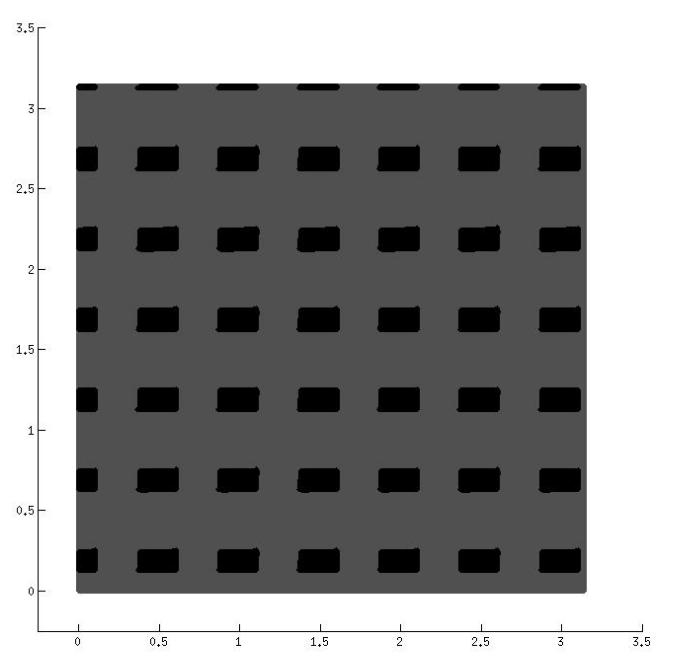
\includegraphics[width=0.5\textwidth]{theta_s_in_uns.jpg}
Now, for a quadratic polynomial, the coefficients corresponding to
complex roots lie within a parabola. This is easily established, 
since, for complex roots of a monic polynomial 
$P(\lambda) = \lambda^2 + x\lambda + y$, we must have
$x^2 - 4y < 0$. Whether an eigenvalue is complex or not is not of
much importance. But for this system of matrices, and indeed it seems for
most such systems, there appear to be regions inaccessible via 
automorphic \glspl{spe}. And, in the 2-dimensional case, such 
regions seem to share two common properties: 
\begin{enumerate}
\item They are conic sections;
\item They lie within this parabola.
\end{enumerate}
For certain systems, for example the system in the previous example,
the entire parabola is inaccessible. A plot of the corresponding
eigenvalues reveals that these inaccessible regions have their 
analogues in the eigenspace. For the present system, since the entire
parabola was inaccessible by automorphic transforms, eigenvalues of all
stable filters are necessarily real.
\begin{figure*}
\centering
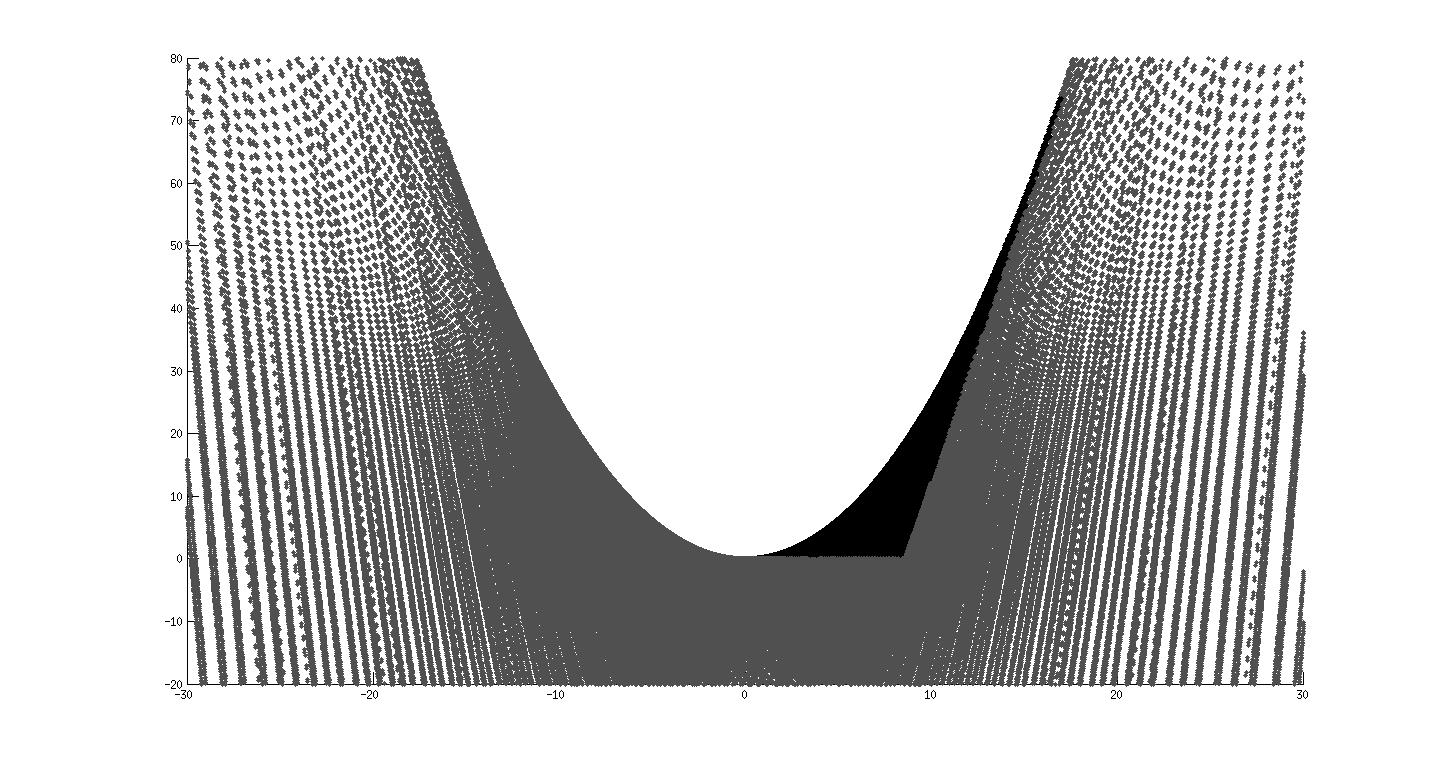
\includegraphics[width=0.9\textwidth]{s_in_uns.jpg}
\caption{Good CPCs (shown in black) and reachable CPCs of a 2D system}
\label{fig:s_vs_us}
\end{figure*}

These special areas also exist for the 3-dimensional case, and
presumably for all dimensions. In the 3-dimensional case, contrary 
to what one might expect, these regions are not cones or
revolutions of conic sections, but have quite arbitrary shapes, with 
symmetry a common feature in the cases examined so far.
The high number of variables involved have made analytical derivation 
of the equations of these regions very difficult. One way to do it 
numerically would be to evaluate the Jacobian at each point. Anywhere 
outside the unreachable region, a point can move in any direction. 
However, at the surface of the region, the point is constrained from 
moving further within the region. Thus the derivative of the 
coordinate vector along these directions would be zero. Hence the 
Jacobian would be rank-deficient, and its determinant would be zero.
This is true independent of the basis chosen for obtaining the Jacobian.
Thus, but determining where the Jacobian is zero, one can approximate 
the surface of the unreachable region.

This method was applied to the present example. For evaluating the partial 
derivatives that make up the Jacobian, a first-order finite difference 
method was used. Then a root-finding algorithm was applied on the Jacobian 
determinant for each grid line. The resultant boundary points are shown in 
\autoref{fig:bound}. The fit (quadratic) is reasonably accurate, as can be 
inferred from the figure. The extra points are due to the gaps in 
calculated points, which arise due to the uniform intervals in which 
the range of values of \gls{t} was divided. The bottom edge, and some 
of the gaps in the space of stable points, which may or may not be 
unreachable, were also detected by this method.
%
\begin{figure*}
\centering
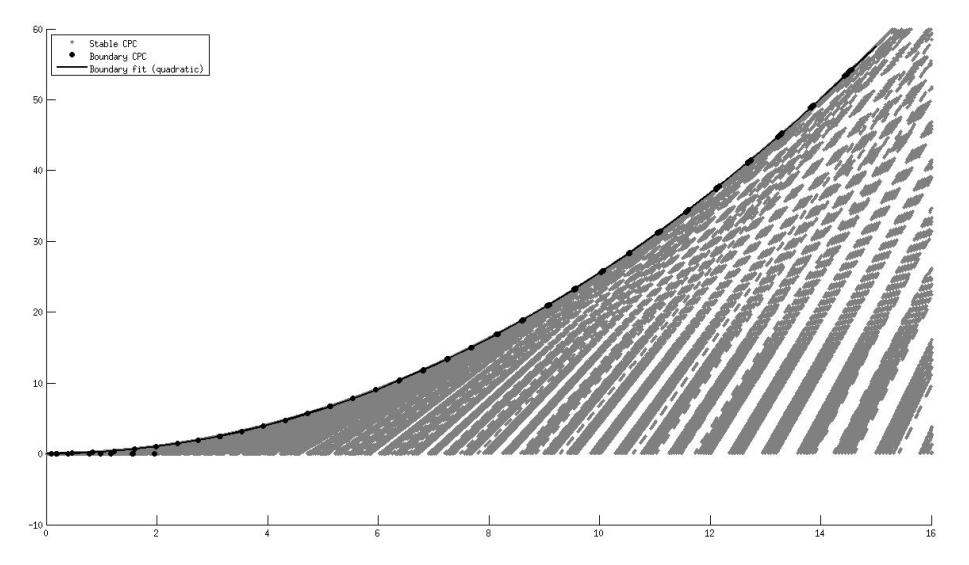
\includegraphics[width=0.9\textwidth]{bound.jpg}
\caption{Scatter of $(\theta_1, \theta_2)$ for good CPCs (in black) over reachable CPCs}
\label{fig:theta}
\end{figure*}
%
\reversemarginpar
\begin{figure*}
\centering
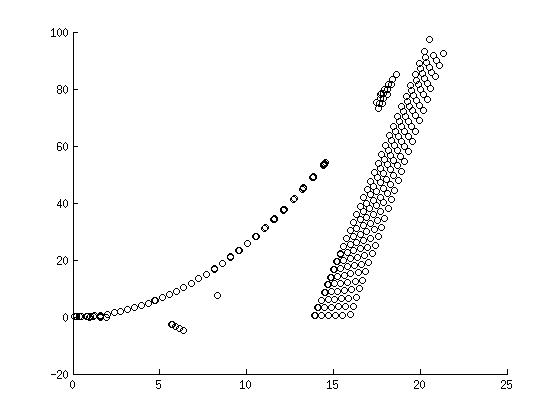
\includegraphics[width=0.9\textwidth]{allbound.jpg}
\caption{Calculated boundary points of unreachable CPC region}
\marginnote{These figures are inside a multicolumn area (using the multicol package. \
So technically, \textsc{technically}, I have satisfied the requirement of having \
a figure span both columns.}
\label{fig:bound}
\end{figure*}
%
\begin{figure*}
\centering
\subfloat[A 3D scatter, seemingly random]{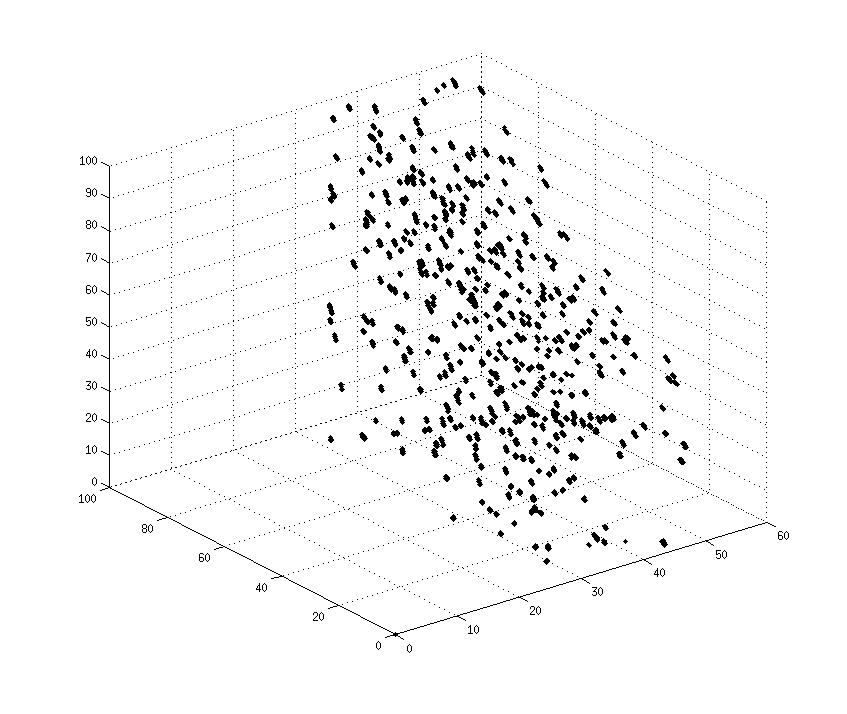
\includegraphics[width=0.48\textwidth]{3d.jpg}}
\subfloat[Projection on the x-y plane, revealing a pattern.]{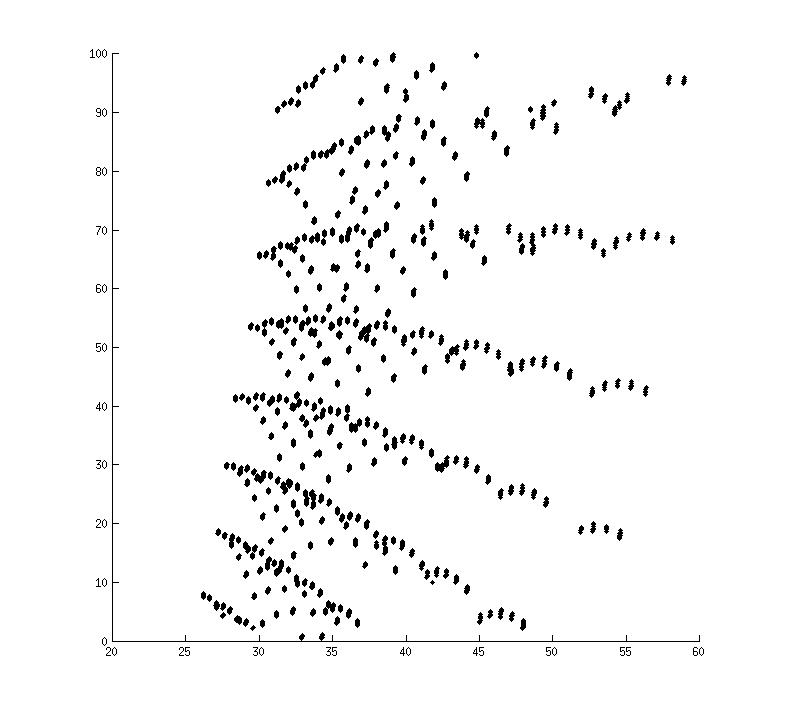
\includegraphics[width=0.48\textwidth]{3d2.jpg}}
\caption{Good CPCs for a 3D system}
\label{fig:3d}
\end{figure*}
\end{multicols}


\newpage
\bibliography{Sources/references}
\printglossary[title={List of Symbols},toctitle={List of Symbols}]
\printglossary[type=\acronymtype] 
\end{document}
